%=======================================================================================%
\chapter{From Protons to Proteins: Methods to simulate the inside of a cell.}
\numberwithin{equation}{chapter}
\label{chap:methods}

The purpose of this chapter is to train those who have studied physics in some of the details they will need to understand the models we use to simulate molecular systems (and the many technical problems they will encounter). An excellent overview which I would recommend as first reading for any new student can be found in an article by Braun et al. \cite{braun2019}. We will go flesh out the physics in some more detail here but this article provides a broader overview of different techniques and resources for where one might be able to find more physical details. 

\section{Quantum Mechanics is Not Tractable at the Scale of Biology.}
Living things are made of atoms and atoms themselves are composed of many particles. The motions of atoms and their constituent particles are governed by quantum mechanics. Unfortunately, performing simulations for the number of atoms involved in proteins and other cellular components at quantum mechanical accuracy is impossible. Hence, we will show how to take the fundamental formulation of atomic interactions in the Schr\"{o}dinger wave equation and apply approximations in order to produce a model which is capable of simulating macromolecular systems at biologically relevant timescales. 

We will gradually integrate upwards, beginning with the interactions in a single atom we will work our way up to a complex macromolecular system with lipids, water, salts and of course, proteins. Ultimately this section rationalises the treatment of atoms as point charges in classical molecular dynamics simulations. 

\subsection{A full quantum mechanical treatment}
Since we are dealing with atoms which are governed by quantum mechanics we must begin our journey upwards with the time dependent form of the Schr\"{o}dinger wave equation. 

\begin{equation}
i\hbar \frac {\partial}{\partial t} \Psi (\textbf{x},t) = \big[ -\frac{\hbar ^2}{2m}\nabla^2 + V (\textbf{x}, t) \big] \Psi (\textbf{x},t) 
\label {schordinger_time_dependent}
\end{equation}

In quantum systems we treat all particles as waves hence the use of the wave function $\Psi (\textbf{x},t)$. The complex amplitude of the wave function $|\Psi (\textbf {x}, t)|^2$ tells us the likelihood of detecting the particle at time $t$ and at place $\textbf{x}$. The term in the brackets correspond to $-\frac{\hbar ^2}{2m}\nabla^2 $ the kinetic energy of the particle with mass $m$ while $V (\textbf{x}, t)$ is the potential energy of the system. Given that the left hand term $i\hbar \frac {\partial}{\partial t} \Psi (\textbf{x},t)$ contains a gradient with respect to time, it governs how the wave function will evolve in time.

When the external potential $V$ has no explicit dependence on time, this equation reduces to the familiar time independent form. 

\begin{equation}
	E \Psi (\textbf{x}, t) = \big[ -\frac{\hbar ^2}{2m}\nabla^2 + V (\textbf{x}) \big] \Psi (\textbf{x}, t) = H \Psi(\textbf{x}, t) 
 \end{equation}

Note that the wave function $\Psi (\textbf {x}, t)$ is still allowed to evolve in time. 

In atomic systems there are two types of particles, nuclei which we will denote with the subscript $i$ and electrons denoted by $e$. In order to treat these elements separately we decompose the Hamiltonian of the system into a few components. 

\begin {equation}
H = \underbrace{T_n + V_{n-n}}_{H_n} + \underbrace{T_e +  V_{e-e} + V_{n-e}}_{H_e}
\end {equation}

Where $T_n$ and $T_e$ denote the kinetic energy of the nuclei and electrons respectively. While $V_{n-n}, V_{n-e}, V_{e-e}$ denote the potential energy for interactions between nuclei, between electrons and nuclei and between electrons respectively.

Since the potential terms all describe charged species, they follow Coulomb's law and have the form.

\begin{equation}
	V_{n-n} = \sum_{i>j} \frac{q_e^2 z_i z_j }{|\textbf{R}_i-\textbf{R}_j|},\quad V_{n-e} = -\sum_{i,l} \frac{q_e^2 z_i }{|\textbf{r}_l-\textbf{R}_i|},\quad  V_{e-e}  = \sum_{l>k} \frac{q_e^2 }{|\textbf{r}_l-\textbf{r}_k|}
\end{equation}

Here the $z_i$ represent the atomic number (and thus the charge) of the $i$th nucleus and $q_e$ is the unit charge of the electron. The reason for the separate coordinates $R_i$ and $r_l$ is to separate out the treatment of nuclei and electrons which will be important once we apply the Born-Oppenheimer approximation.

Meanwhile, the kinetic energy terms are of the form 

\begin {equation}
T_n = - \sum_i \frac{\hbar^2}{2M_i} \nabla_i ^2,\quad  T_e = - \sum_l \frac{\hbar^2}{2m_e} \nabla_l ^2
\end {equation}

$M_i$ represents the mass of the $i$th nucleon and $m_e$ represents the mass of an electron. The operator $\nabla^2 = \frac{\partial^2}{\partial x^2} + \frac{\partial^2 }{\partial y^2} + \frac{\partial^2}{\partial z^2} $. The separate subscripts $i$ and $l$ are due to the different coordinates which we use to denote the positions of the nuclei and the electrons. The reason for this will become clear when we derive the Born-Oppenheimer approximation to separate the wave functions and treat them separately.

\subsection{The Born-Oppenheimer approximation.}
In order to reach the Born-Oppenheimer approximation we start with the observation that electrons have a mass 3-4 orders of magnitude smaller than the nuclei. This motivates two simplifications. The `clamped nuclei assumption" where we solve the Schrodinger equation whilst nuclei are fixed in space and do not move. And a related assumption known as the "adiabatic assumption" which postulates that the electrons will respond instantaneously to any changes in the positions of the nuclei. Combining these physical approximations we derive the ``Born-Oppenheimer approximation" for the Schrodinger equation which can be used to simplify calculations involving several atoms at once. 

We begin the derivation by examining the time-independent form of the electronic Schrodinger wave equation where the nuclei are fixed at positions $R_i$. 

\begin{equation}
	H_e(\bold{r}_l, \bold{R}_i)  \psi_e (\bold{r}_l,\bold{R}_i)  = E_e(\bold{R}_i) \psi_e (\bold{r}_l,\bold{R}_i) 
\end{equation}

Fixing the nuclei in this way gives the ``clamped nuclei" approximation \cite{sherrill}. To solve the wave function for the whole system $\Psi_{tot}$ we use an \textit{ansatz} which decomposes the wave function with an electronic basis into two components: $({\psi_e})_k$ and $({\psi_n})_k$ which are the $k$th eigenfunction solutions to $H_e$ and $H_n$ respectively.

\begin{equation}
	\Psi_{tot} (\bold{r}_l,\bold{R}_i, t) = \sum_{k=0}^\infty {\psi_e}(\bold{r}_l, \bold{R}_i)_k\ {\psi_n}(\bold{R}_i)_k
\end{equation}

Note that there is an implied direct product between the wave functions $\psi_e(\bold{r}_l, \bold{R}_i)$ and $\psi_n(\bold{R}_i)$. When we substitute this expression into the full Schrodinger equation \ref{schordinger_time_dependent} we find the following expression for the $k$th nuclear eigenfunction \cite{miller1976} 

\begin{equation}
	i \hbar \frac{\partial} {\partial t} {\psi_n(\bold{R}_i)}_k = \Big[- \sum_i \frac{\hbar^2}{2M_i} \nabla^2_i  + {E_e} (\bold{R}_i)_k\Big] \psi_n (\bold{R}_i)_k + \sum_j C_{kj} \ {\psi_n(\bold{R}_i)}_j 
	\label{adiabatic_approx}
\end{equation}

Where we have coupled the electronic wave functions to each other with the operator 

\begin{equation}
	C_{kj} = \int ({\psi_e})_k ^* \Big[\sum_i\frac{\hbar^2}{2M_i}\nabla^2_i\Big] ({\psi_e})_j d\bold{r}  + \frac{1}{M_i}\sum_{i}\bigg[ \int({\psi_e})_k ^* [-\hbar i \nabla_i]({\psi_e})_jd\bold{r}\bigg] [-\hbar i \nabla_i]
\end{equation}

Using the ``adiabatic assumption" \cite{miller1976} the off-diagonal terms of $C_{kj}$ can be set to $0$. This completely decouples the wavefunction into two components 
\begin{equation}
	\Psi_{tot} (\bold{r}_l,\bold{R}_i, t) = {\psi_e}(\bold{r}_l, \bold{R}_i)_k\ {\psi_n}(\bold{R}_i,t)_k
\end{equation}

Since all cross terms from the direct product can be ignored. With the further assumption that the diagonal terms $C_{kk}$ can also be ignored because they are 4 orders of magnitude smaller than the other terms in \ref{adiabatic_approx} \cite{sherrill}.

We now write the Born-Oppenheimer approximated wave equation for an atomic system.  


\begin{equation}
	i\hbar \frac{\partial}{\partial t} \psi_n(\bold{R}_i)_k = \big[ -\sum_i \frac{\hbar^2}{2M_i} \nabla^2_i + E_e(\bold{R}_i)_k\big] \psi_n(\bold{R_i})_k 
\end{equation}

By rearranging this equation and taking derivative we can see how to use Newton's equations of motion to calculate the forces on the nuclei from the surrounding electric potential 

\begin{equation}
	M_i \ddot{\bold{R}}_i (t) = -\nabla_i E_e (\bold{R_i})
	\label{Newtons_equations}
\end{equation}

By choosing an appropriate time-step one can simply iteratively solve this equation of motion to understand the dynamics of an atomic system. The nuclei will move according to their relative positions to each other and the electron clouds will rearrange in response to that motion. There is no need to calculate the interactions between the nuclei and the electrons. This is sufficient accuracy to simulate many physical phenomena with the notable exception of energetic, fast interactions between nuclei and electrons such as spectroscpic phenomenon \cite{sherrill}. 
%\begin{equation}
%	(H_n + H_e + V_{n-e})  (\psi_e (\bold{r}_l,\bold{R}_i) \psi_n(\bold{R}_i)) =  (E_n  + E_e)(\psi_e (\bold{r}_l,\bold{R}_i) \psi_n(\bold{R}_i) ) 
%\end{equation}
%

%disregard $T_e$, $V_{n-e}$ and $V_{e-e}$ as they will be close to 0 compared to $T_n$ and $V_{n-n}$.

%In the case of hydrogen we lose an order of magnitude so the approximation is less valid, especially at room temperature. CITATION NEEDED


%
%\begin {equation}
%\Psi(R_i,t) = \psi_e (r_l,R_i) \psi_n(R_i,t)
%\end {equation}
%
%The BO assumption means that we can neglect the cross terms from this separation and treat each wave function independently.
%
%\begin {equation}
%T_n + T_\Psi(R_i,t) = \psi_e (r_l,R_i) \psi_n(R_i,t)
%\end {equation}


\section{Classical MD, Molecular Motions Without Quantum Mechanics}
The Born-Oppenheimer approximation gives rise to Hartree-Fock methods and density functional theory (DFT). These more sophisticated physical methods allow us to simulate the the organisation of electron clouds around small molecules, finding broad applications in chemistry and materials science \cite{vanmourik2014}. We can derive the energy profile of certain degrees of freedom within the molecule such as the energetics of stretching out a bond or twisting a dihedral angle. These can be useful when designing novel materials. 

However, even with these approximations simulating a large number of atoms is still not computationally tractable. State of the art DFT methods can only simulate up to a few 10s of thousands of atoms \cite{luo2020} and scales as $O(N^3)$ \cite{kresse1996}. This is not sufficient to simulate proteins and their surrounding solvation environment. So, we must use another round of approximations to reach the spatial and time scales necessary to simulate biological molecules. We do this by creating a set of mathematical functions the calculations further. Here we use a set of virtual springs and other simple models for the energetic interactions between atoms. This creates what's known as an effective potential. So named because it effectively approximates the behaviour of the full quantum mechanical system.

This formulation gives us classical molecular dynamics sometimes referred to as molecular mechanics. The aim of the classical forcefields discussed here is to use \textit {ab initio} MD as a target to approximate. 

The CHARMM effective potential employed in this work is similar to those found in all common all-atom molecular dynamics forcefields. The same  functional forms are used in other forcefields such as AMBER, GROMOS and OPLS but with different parameters and design philosophies. [CITATION NEEDED]

We split up the molecular potential into several components dealing with the energies from covalent bonds, including bond stretching, twisting and pinching. As well as energies associated with the forces that atoms exert on each other when they are not bonded together. Namely Coulomb forces due to electric charges on the atom and attractive Van Der Walls interactions and repulsion due to Pauli Exclusion the latter two forces are combined into one term we will analyse in detail $U_{LJ}$.

\begin{equation}
	U_{MM} = \underbrace{U_{LJ} + U_{Coulomb}}_{U_{non-bonded}} + \underbrace{U_{bonds} + U_{angles} + U_{dihedrals} + U_{impropers}}_{U_{bonded} }
	\label{CHARMM_effective_potential_eq}
\end{equation}

Interestingly, the bonded terms may all reasonably be approximated by harmonic springs. 

\begin{equation}\label{bonded_eqs}
	\begin{aligned}
	U_{bonded} = \sum_{bonds} k_{b} (b-b_0)^2 + \sum_{angles} k_\theta(\theta-\theta_0)^2+ \sum_{Urey-Bradley} k_u(r_{UB}-r_{UB_0})^2   \\ + \sum_{dihedrals} k_\varphi (1+\cos(n \varphi - \delta)) + \sum_{improper-dihedrals}  k_{\phi} (\phi - \phi_0)^2 
\end{aligned}
\end{equation}

Here, the $k_i$ terms correspond to the strength of the harmonic restraint for that parameter. The $0$ subscript denotes the equilibrium position for that parameter. Even though this formulation is quite simple, it has empirically been shown to be a reasonable approximation for the potential energy functions of quantum mechanics in covalently bonded bonded species. Examples can be seen in figure \ref{morse_potential}.

\begin{figure}
	\begin{center}
	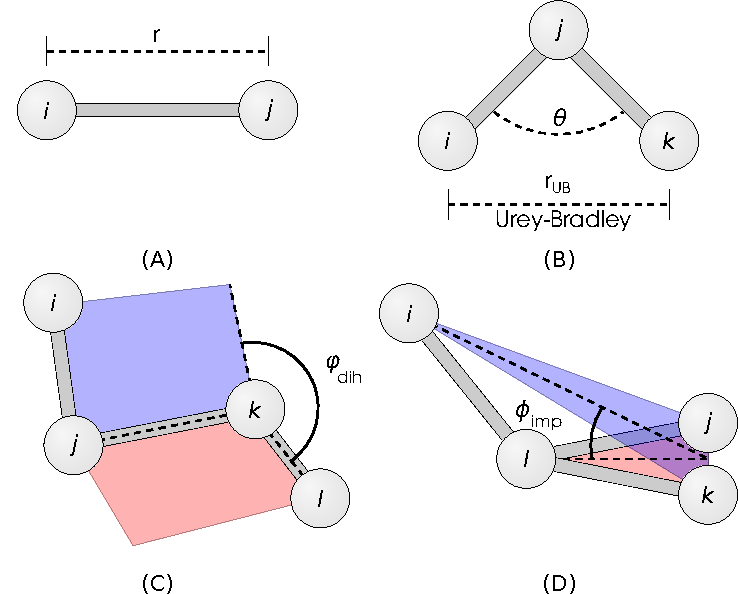
\includegraphics[width=10cm]{figures/bonded_interactions.pdf}
	\end{center}
	\captionsetup{singlelinecheck = false, justification=raggedright}
	\caption[The Bonded Interactions Calculated In Classical Forcefields]{\textbf{The Bonded Interactions Calculated In Classical Forcefields.}}{
	(A) The energy of Bond Stretching is approximated as a harmonic oscillator with respect to their separation $r$. (B) Angles between neighbouring covalently bonded atoms are also approximated as a harmonic oscillator with respect to the angle $\theta$. In some forcefields such as CHARMM there is a correction term for these angular interactions known as Urey Bradley forces. This is calculated using the separation between the non-bonded atoms $i$-$k$ in the triplet with the parameter $r_{UB}$. (C) The dihedral angle between four atoms is calculated by constructing two planes. Each plane is constructed to contains three of the four atoms in the set. One plane encompasses atoms $i, j$ and $k$ here colored in blue and the other plane contains the $j$, $k$ and $l$ atoms colored in red. The dihedral angle is then calculated by taking the angle between these two planes along the line they intersect, the line formed by the $j$-$k$ bond. (D) The improper dihedral angles enforce the planarity of a molecular configuration. A plane is constructed to contain the $i$, $j$ and $k$ (blue) atoms and another plane is constructed to contain the $j$, $k$ and $l$ atoms (red). The improper angle is then calculated as the angle between these two planes. }
	\label{charmm_bonded}
\end{figure}


In classical forcefields the non-bonded interactions are expressed using the Couloumb's law because the partial charges assigned to each atom and the Lennard-Jones potential to approximate the interactions arising from both Pauli exclusion and Van Der Walls Interactions.


\begin{equation}\label{nonbonded_eqs}
	\begin{aligned}
		U_{non-bonded} = \underbrace{\sum_{i>j} \epsilon_{ij} \Big( \Big(\frac{\sigma_{ij}}{r_{ij}}\Big)^{12} - \Big(\frac{\sigma_{ij}}{r_{ij}}\Big)^{6} \Big)}_{U_{Lennard-Jones}} - \underbrace{\sum_{i>j} \frac{q_i q_j } {r_{ij}}}_{U_{coulomb}}
	\end{aligned}
\end{equation}


The $\sigma$ parameter denotes the location of the local minima in the Lennard-Jones potential. This is the optimum distance that two atoms will rest against each other in the absence of other effects. The $\epsilon$ parameter denotes the depth of the potential well, or how stable the two atoms will be in the minimum energy configuration. This is very important for certain physical parameters such as osmotic pressure  \cite{yoo2018a}

Conversely, the partial charges in a system have the greatest influence on the solvation energy.

By focussing on these two physical parameters we can isolate and improve the non-bonded parameters.

\begin{figure}
	\begin{center}
	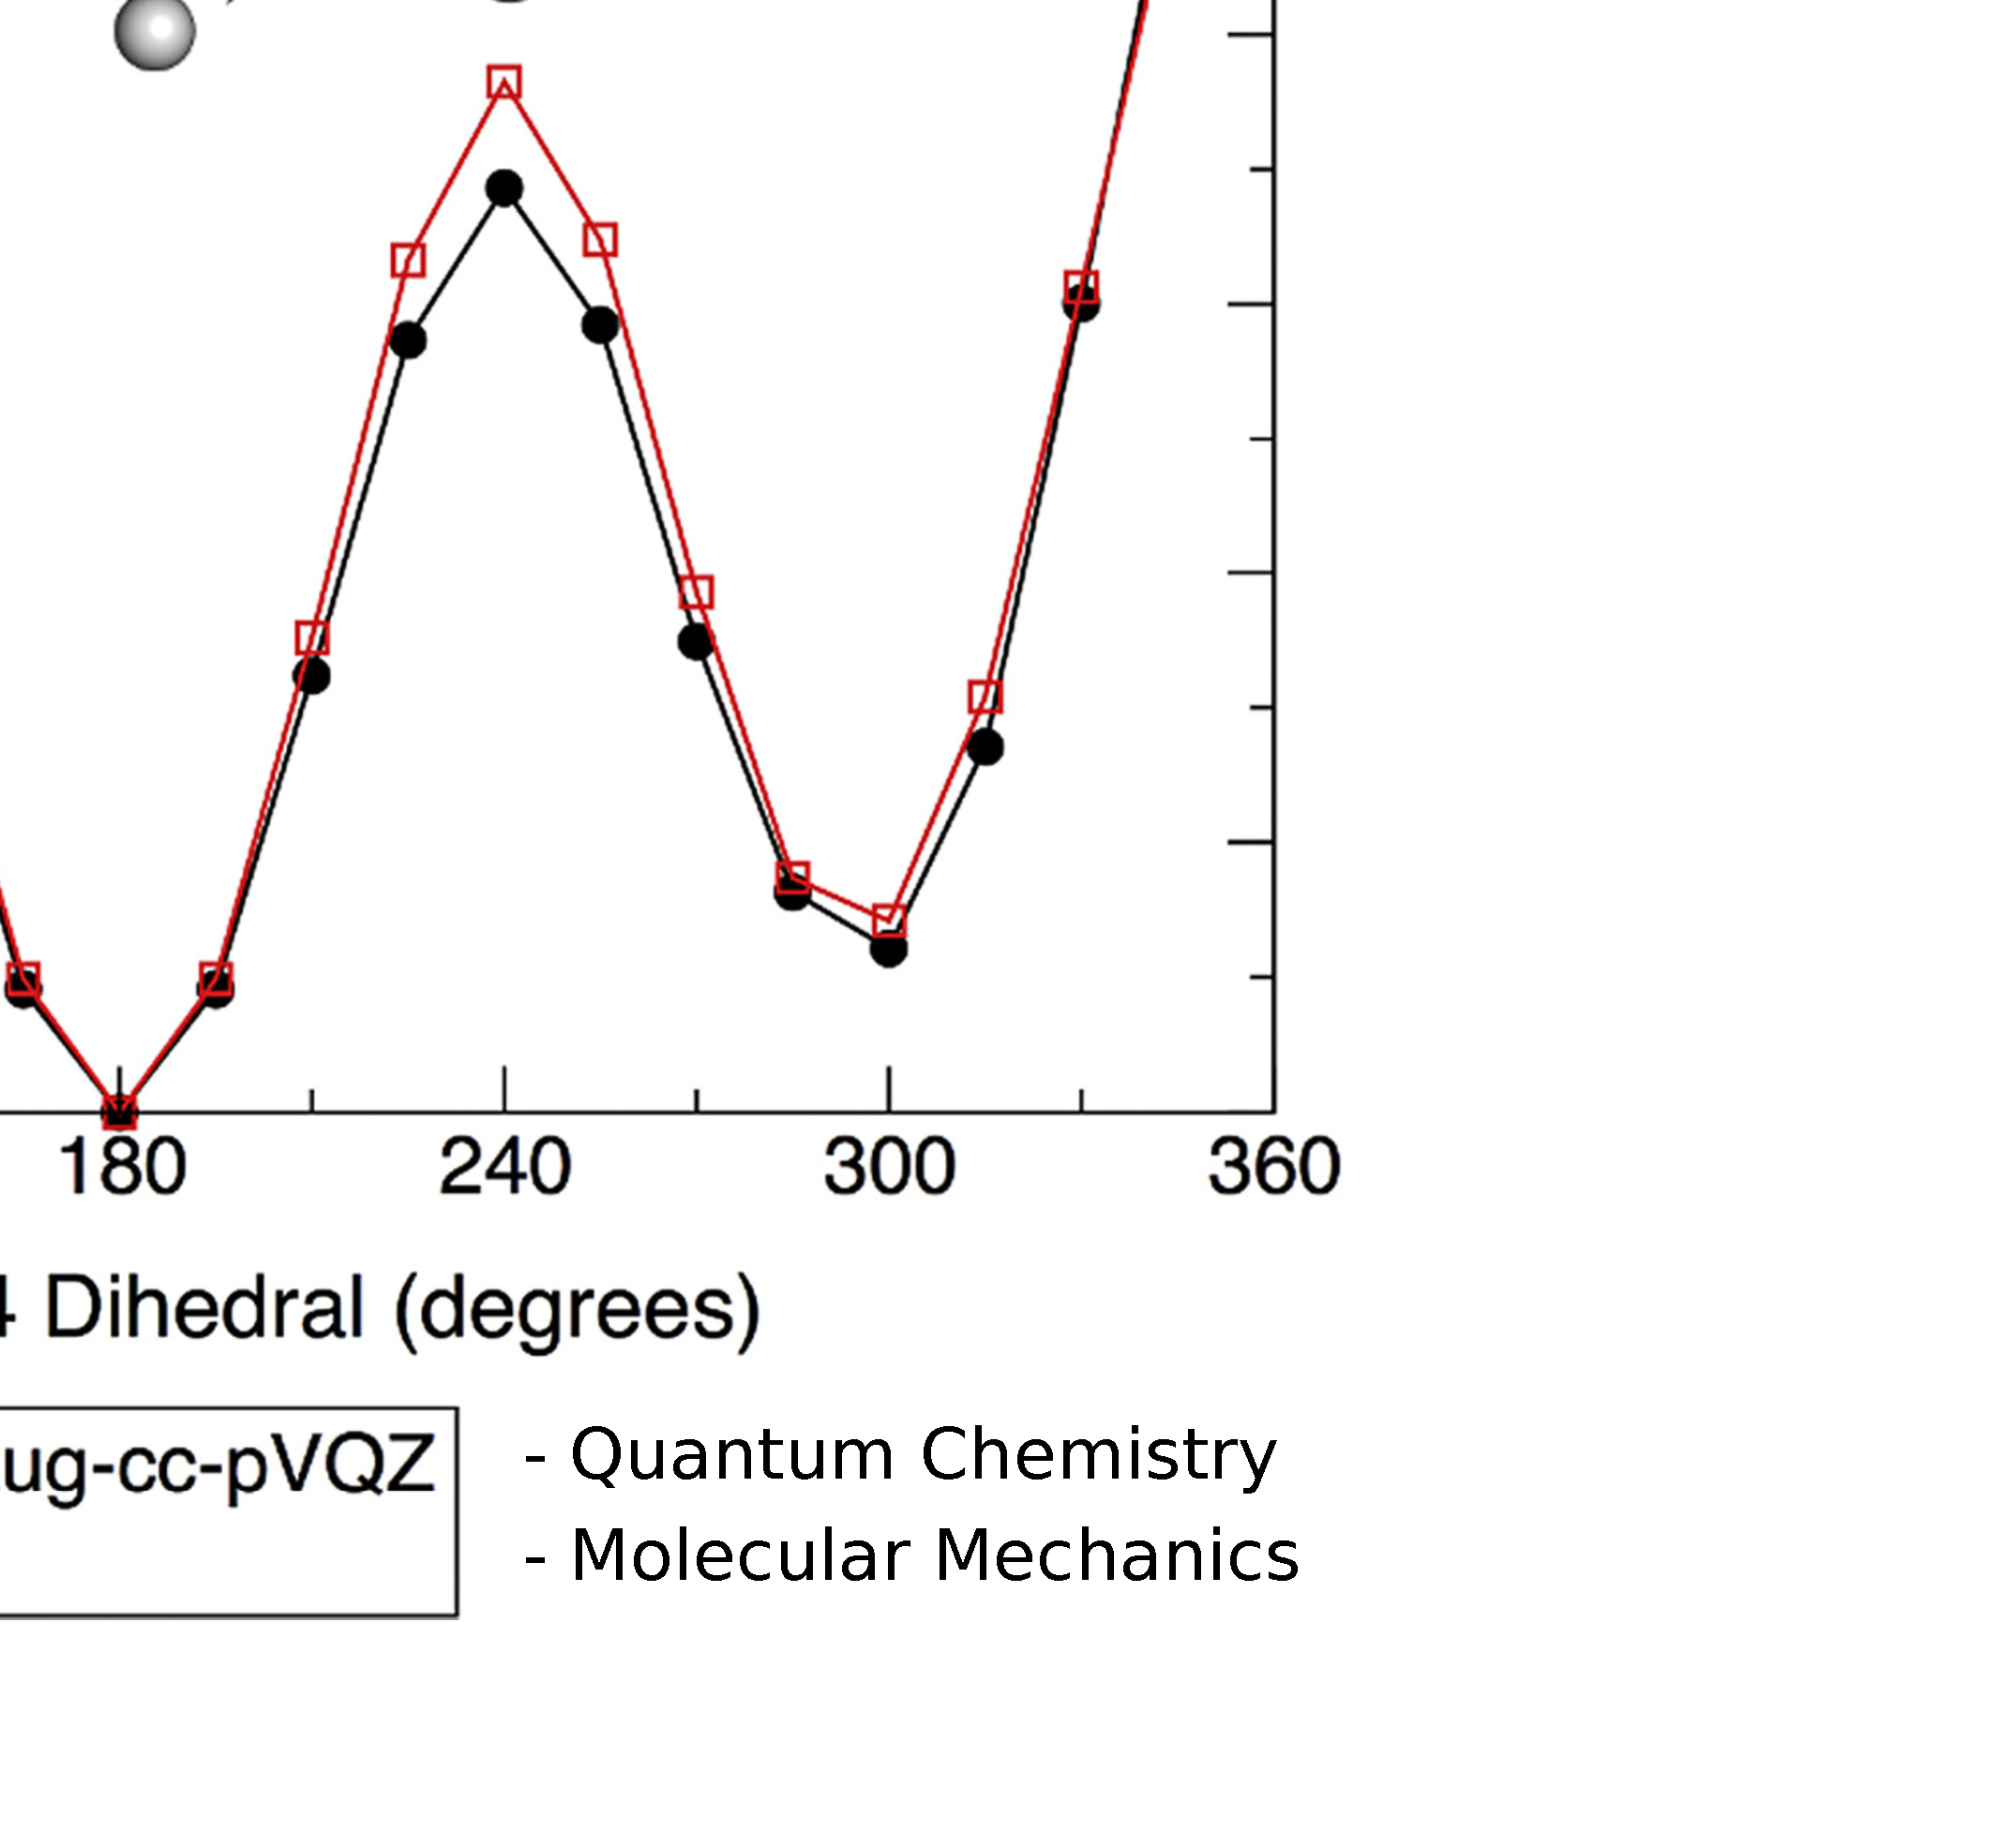
\includegraphics[width=\textwidth]{figures/QM_MM_compared.pdf}
	\end{center}
	\captionsetup{singlelinecheck = false, justification=raggedright}
	\caption[Comparison Between Potentials in Quantum and Classical Forcefields] {\textbf{Comparison Between Potentials in Quantum and Classical Forcefields}}{ A) The Morse potential was formulated to approximate the potential the potential energy surface associated with the stretching of covalent bonds (blue). At low temperatures (the ground state, $v=0$) like those found in classical MD there is good agreement between the Morse potential and the harmonic oscillator (green). Credit Mark Somoza 2006 B) Here the potential of the dihedral angle between the atoms C1,C2,C3 and C4 in a butane molecule is calculated using two methods: Quantum Chemical calculations and approximations using the functional form in \ref{bonded_eqs} \cite{lemkul2020}. Note how the appropriate choice of $k_\varphi$, $n$ and $\delta$ have closely approximated the results the more accurate quantum mechanical calculations.}

	\label{morse_potential}
\end{figure}

\subsubsection{The Lennard-Jones Potential}
\begin{figure}
	\begin{center}
		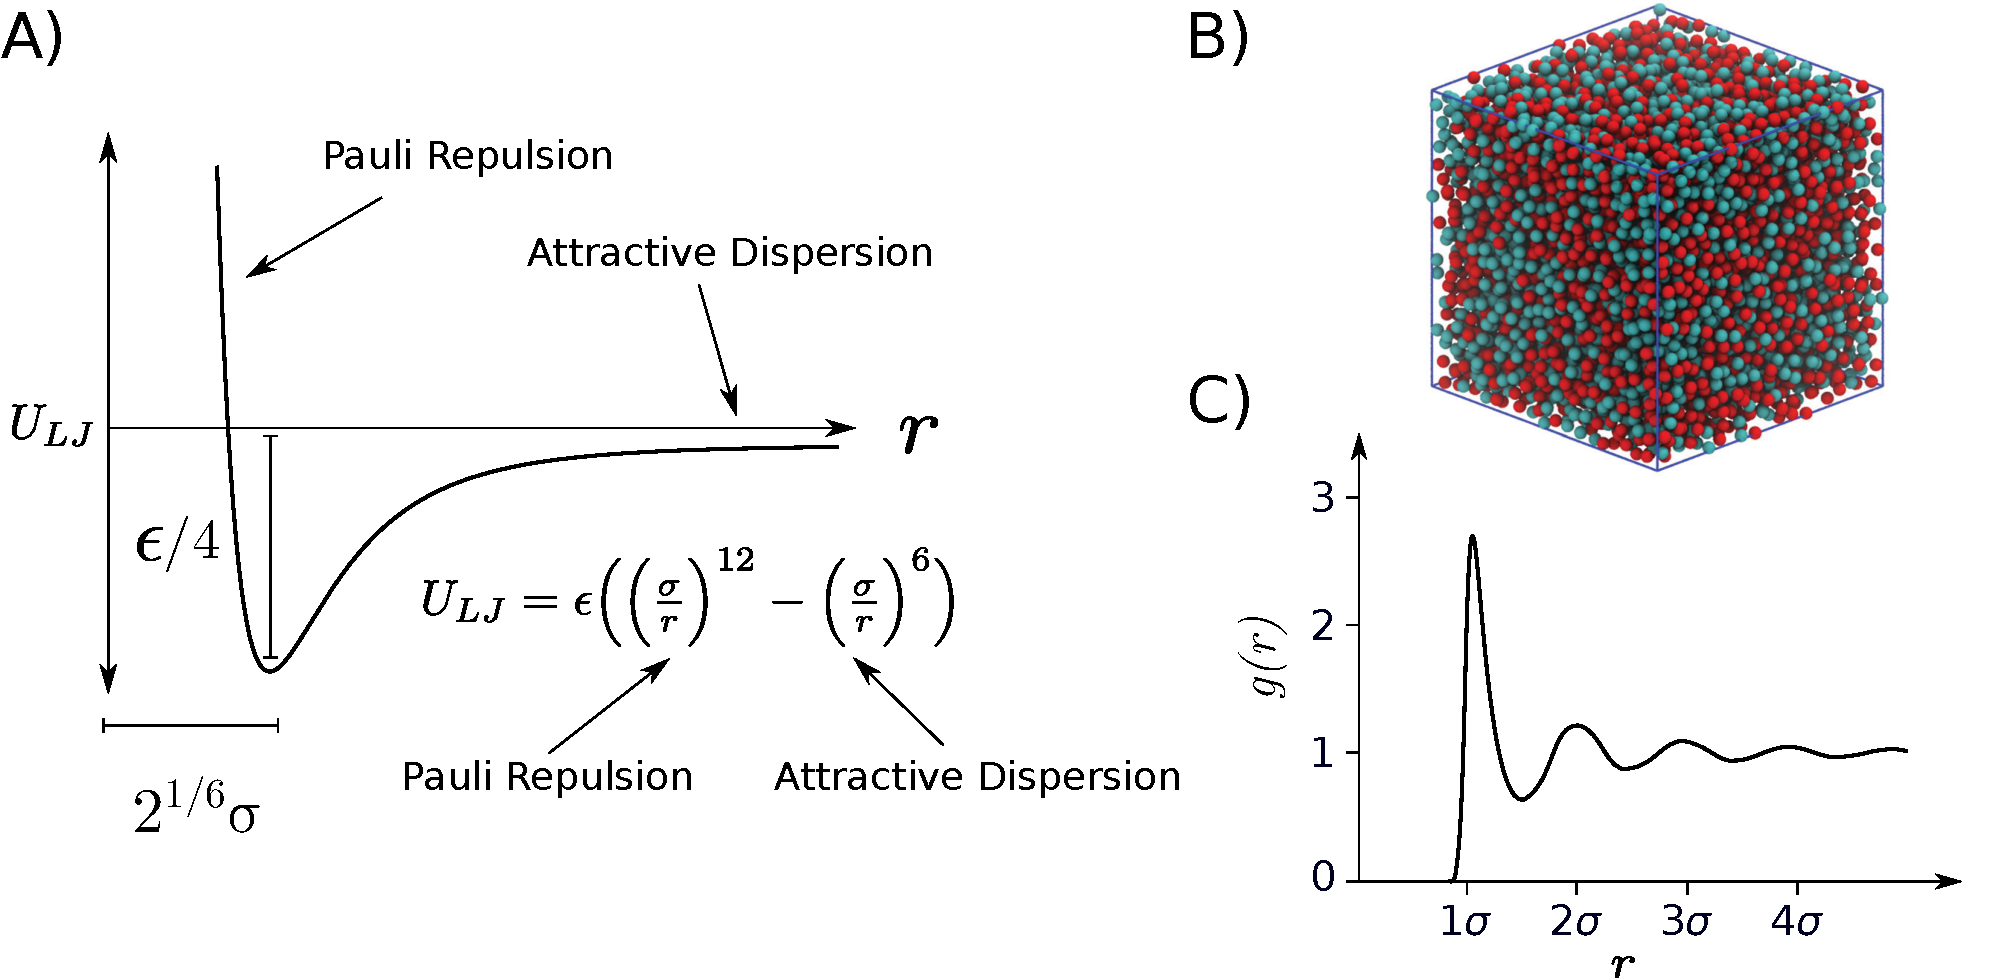
\includegraphics[width=\textwidth]{figures/LJ_figure.pdf}
	\end{center}
	\captionsetup{singlelinecheck = false, justification=raggedright}
	\caption[The Lennard-Jones Potential] {\textbf{The Lennard-Jones Potential}}{A) The Lennard-Jones potential function has two regimes, the far region one dominated by attractive dispersion forces and the close region dominated by repulsion. In the case of atomic systems this is due to the Pauli exclusion principal. B) An example of a fluid modelled with Lennard-Jones particles \cite{chari2019}. C) The radial distribution function ($g$) for a Lennard-Jones fluid \cite{morsali2005}. Note that the peaks in the distribution are roughly 1 $\sigma$ apart. }
	\label{Lennard-Jones_figure}
\end{figure}

\subsection{Philosophy of Different Molecular Mechanics forcefields.}
At the time of writing, the four popular forcefields for the simulation of biomolecules are: AMBER, CHARMM, GROMOS and OPLS. Each of these have a slightly different philosophy in their formulation. They may be bottom up, as in the case of AMBER and CHARMM or top down, in the case of GROMOS and OPLS. Bottom up forcefields take the results from quantum \textit{ab initio} calculations and approximate them with the functional form mentioned above. Conversely, top down forcefields take experimental measurable such as Osmotic pressure, solvation energy. This philosophy is closest to physics 


\subsection{Controlling the Temperature and Pressure in a Simulation}
Living things generally die if you put them in the freezer, as a rule, they also do not survive in an autoclave. As such, to correctly understand their function with simulations we not only need to correctly calculate the forces being exerted on every atom in their bodies but we must also keep those virtual bodies at realistic temperatures and pressures. In general, we seek to approximate the environment conceptualised as an open topped test-tube sitting in a pressure and temperature controlled laboratory. To do this, we make use of some statistical ensembles chosen for their performance in regulating the thermodynamic quantities in a simulation and their computational expense.  

\subsection{Berendsen Thermostat}
Remember that the temperature of a system is a direct function of the velocity of its constituent atoms. So by regulating the ensembel of velocities we can control the temperature. The simplest way to do this dynamically is taking the equations of motion and add both a damping term, to lower the temperature and a random acceleration to raise the temperature. 
Reference temperature $T_0$ 

\begin{equation}
	m_i  \dot{v} _i = F_i + m_i \gamma_i \bold{v}_i + R(t)
\end{equation}

Here $gamma_i$ is the damping factor, $m_i$ is the mass of the particle and $R(t)$ is a random variable to the kick.


\subsection{Berendsen Barostat}

\subsubsection{Nos\'e Hoover Thermostat}
The themostat begins by choosing the velocities of the atoms within the system from a Maxwell-Boltzmann distribution. Despite starting from the same cartesian coordinates, this means that two replicate simulations will immediately begin from different points in phase space. They will quickly diverge, raising questions around how long one should run a simulation and how many replicates they should run . A good rule of thumb


\subsection{Periodic Boundaries to Simulate the Inside of Cell}
\begin{figure}
	\begin{center}
		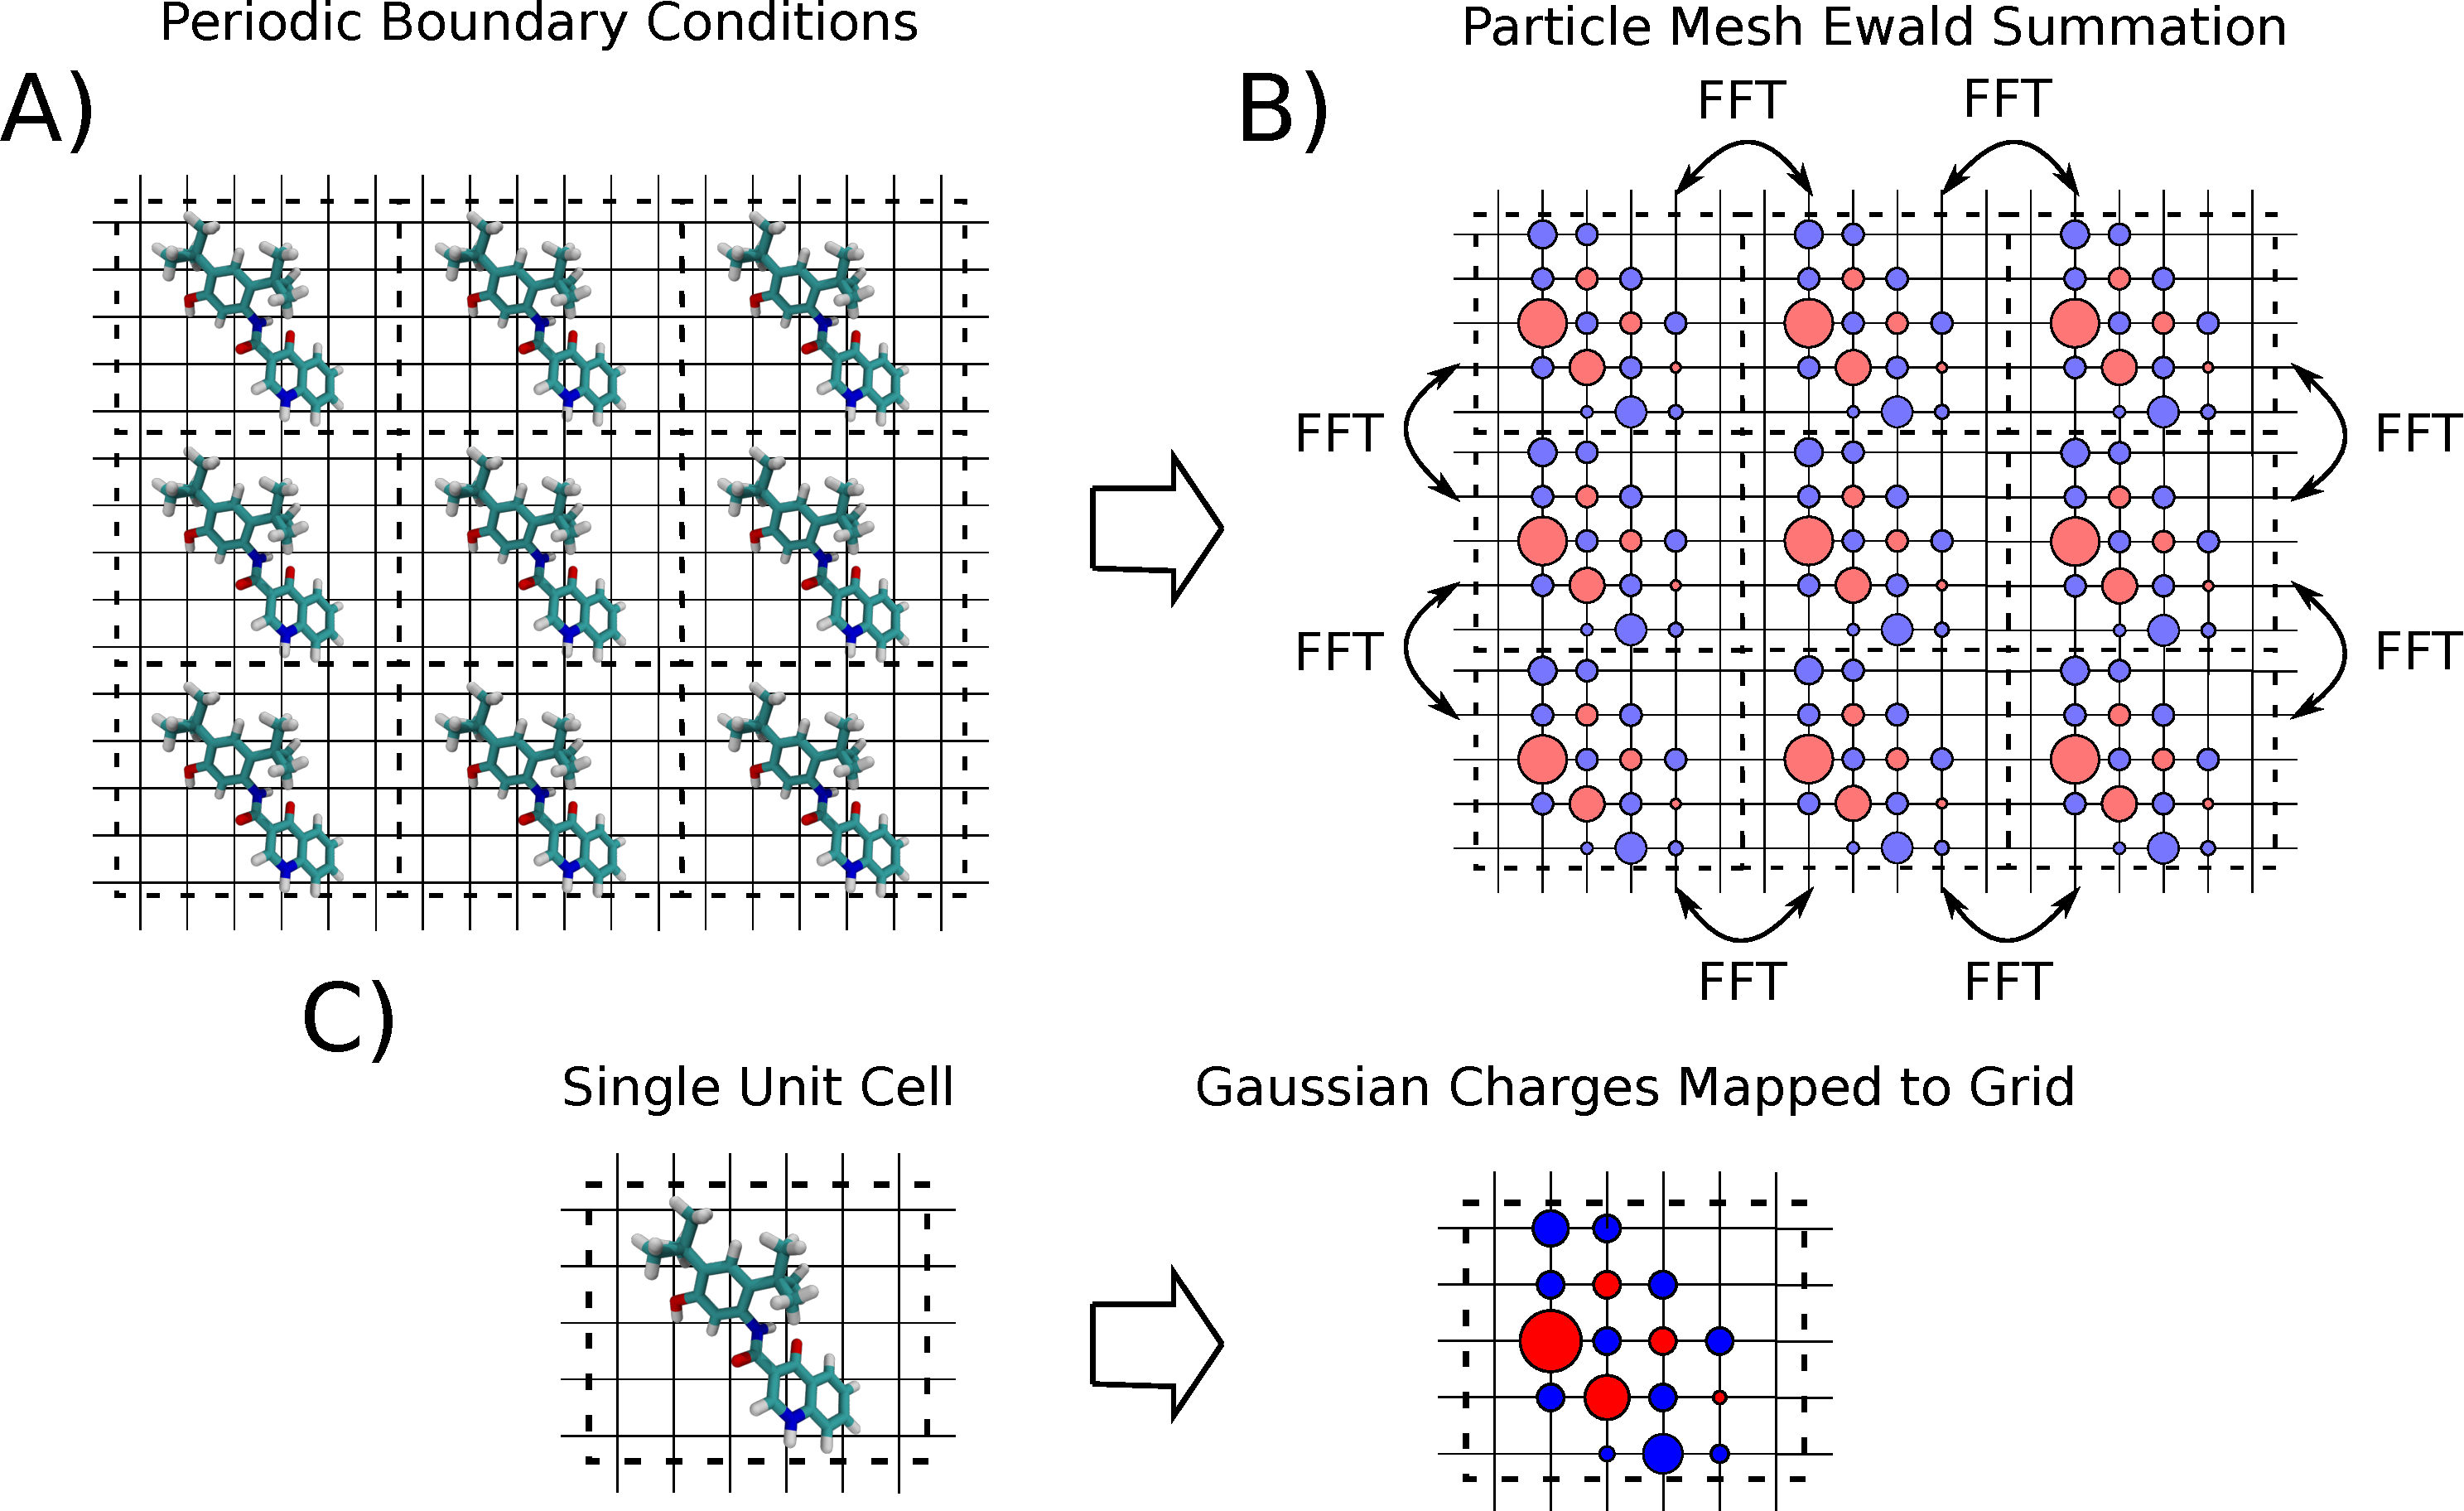
\includegraphics[width=\textwidth]{figures/PME_miro.pdf}
	\end{center}
	\captionsetup{singlelinecheck = false, justification=raggedright}
	\caption[Particle Mesh Ewald Summation] {\textbf{Particle Mesh Ewald Summation}}{A)The molecular system is repeated infinitely along all axes, when atoms reach the edge of the simulation box they are allowed wrap around to the other side of the box. B) The charges in the infinite periodic system are approximated as Gaussian functions on a grid. Then the potential on these screening charges is calculated via a Fast Fourier Transform (FFT). C) A more detailed view of the charge mapping procedure. A series of Gaussian charges centered on the grid points are constructed to reflect the potential from the point charges in the unit cell. }
	\label{PME_illustration}
\end{figure}

Inside cells, proteins are immersed in a large solvation environment composed of water and salts \cite{phillips2012}. In order to avoid artefacts we have to replicate this environment somehow\cite{ross2018}. We could make a simulation box large enough to replicate the behavior of a bulk solvent, but even with a large simulation box we can still observe artifacts associated with the vacuum at the boundaries \cite{gapsys2020}. So, to avoid these boundary effects we use periodic boundary conditions (PBCs), allowing atoms to move between images in the simulation box \ref{PME_illustration}. This replicates the molecular system infinitely in every direction. 

Using PBCs might remove vacuum from our molecular system but now we have a different problem. Effectively, with the PBCs, we have created a system with an infinite number of atoms. We have to somehow limit the number of computations we perform. We could simply truncate the calculation of interactions $U_{non-bonded}$ after a certain cutoff distance. This is not an issue for $U_{LJ}$ because the $1/r^6$ and $1/r^{12}$ terms in \ref{Lennard-Jones_figure} decay very quickly for large $r$. Inaccuracies due to this approximation can be further ameliorated with the use of a smooth switching function \cite{klauda2007}\cite{venable2009}. On the other hand, the $1/r$ dependence in $U_{coulomb}$ scales much more slowly so truncating it leads to many artefacts in the simulation.\cite{auffinger1995}\cite{perera1995}\cite{roberts1994}\cite{delbuono1996}\cite{essmann1995}. Note that this periodicity requires that the unit cell is neutral, else the contribution of potential energy from $U_{coulomb}$ will be infinite, leading to artifacts \cite{hub2014}.

To avoid these artefacts and limit computational intensively of our calculations we use a clever scheme known as Particle Mesh Ewald Summation. Interestingly, this scheme ends up scaling better than the pairwise summation in equation \ref{nonbonded_eqs} might imply. The direct summation scales with computational complexity of $O(N^2)$  with the number of atoms while the infinite PME scheme scales as $O (N\log N)$ \cite{darden1993}, though there are some further considerations for large systems on parallel architectures \cite{hardy2015}. Even with these sophisticated algorithms, the calculation of electrostatic potential still represents the largest computational bottle-neck in classical MD \cite{hardy2015}.

For a detailed review of different Particle Mesh Ewald Summation methods and the mathematics behind the method see \cite{shan2005}. A brief outline of the Smooth Particle Mesh Ewald summation is given below 

\begin{enumerate}
	\item Point charges from atoms are interpolated onto a grid using B-spline interpolation functions. This procedure is demonstrated in figure \ref{PME_illustration}.
	\item The charge density functions in the grid are transformed into $k$-space using Fast Fourier Transforms.
	\item The Poisson equation is solved numerically in $k$-space.
		\begin{equation}	
			\nabla^2\tilde{U} = \tilde{\rho}(\bold{k})
		\end{equation}	
		Where $\tilde{U}$ is the component of $U_{coulomb}$ we solve for in $k$-space and $\tilde{\rho}$ is the fourier transform of the smooth scalar function for the interpolated charge densities. 
	\item An inverse Fourier transform is calculated to calculate solution to the Poisson equation in real space. 
	\item Now that $U_{coulomb}$ is known at every position in the unit cell we can move atoms according to this potential using Newton's second law.
\end{enumerate}

%\begin{equation}
%	\label {couloumb_eq}
%	U_{coulomb} =  \frac{1}{2} \sum_{i,j=1}^N \sum\limits_{\substack{\bold{n}\neq \bold{0}, \\i\neq j}}\frac{q_iq_j}{|\bold{r}_i -\bold{r}_j -\bold{n} L  |} 
%\end{equation}
%
%The variable $\bold{n} = (n_x,n_y,n_z) \in \mathbb{Z}_3$  is used to locate the locate the periodic image of an atom in the unit cell. If an atom is located at $\bold{r}$ it will have a periodic image located at $\bold{r} + \bold{n} L$.
%
%\begin{equation}
%	\label {Poissons_equation}
%	\nabla^2 U(\bold{r})  = \rho (\bold{r})
%\end{equation}
%

\subsection{The Process of Preparing a Simulation}
The process of taking a molecular structure and putting it in a cellular environment to simulate it at physiological temperatures is both an art and a science. It's a science because a biophysicist must be aware of the many tricks that structural biologists use to image a macromolecular complex. But it's an art because accounting for those tricks and modifications is rarely straight forward. How do you build a missing loop? What charge state is an amino acid most likely to take during the physiological context.

\subsection{Short Comings of Classical MD}
The short comings of classical molecular dynamics fall into two classes whose solutions stand opposed to one another. These are the accuracy of the chemical forcefields outlined above and the inability of modern computers to deliver enough samples of the energy landscape to collect sufficient statistics for rigorous conclusions. The issue is that, as the above physical formulation might indicate. The more accurate the forcefields, the more computationally expensive. And so the solutions to the two are constantly in tension with one another. In the next section we will explore the current efforts to bring solutions.

\subsubsection{The Problem with Forcefields}
These approximations are not without a cost to accuracy. In certain situations, many of which are biologically relevant, it has been shown that quantum effects such as polarisation play an important role in the dynamics of the system. This has been demonstrated in the literature for Gramicidin where polarisable forcefields are able to more accurately reproduce the experimental results of current.

The other context where polarisation is important to consider are on divalent ions. Here, the solvation energy is underestimated due to the consistent lack of polarisation, making investigations of these biologically important chemical species difficult.

However, for most situations, particularly those involving bulk water and protein motions Molecular Dynamics is proving to be an invaluable tool for investigating the properties of biological systems CITATION NEEDED. Sadly, it should be kept in mind that classical MD is not able to simulate any chemistry such as forming and breaking or the change a change in profanation state. Such interactions require considerations of Quantum Mechanics which are computationally expensive.

There are several efforts to correct address some of the above issues. These include the inclusion of the effects of polarisation, the most popular methods at the moment being adding a massless drude oscillator as an extra bead to most(?) atoms as in the CHARMM drude forcefields, championed by the Mackerell lab and the use of forcefields such as AMOEBA which explicitly calculate the dipole and quadrupole moments of each atom. These both substantially increase computational cost but have displayed much better agreement with experiments in biological systems where classical forcefields have been shown to fail \cite{ngo2021}. 

Ultimately, the functional form in equation \ref{CHARMM_effective_potential_eq} used by classical forcefields does not have sufficient degrees of freedom to address all possible chemical contexts. Careful consideration must always be given to whether the forcefield is being used in a faithful way to the situations it was intended to accurately represent. So long as the user is aware of the situations where a given forcefield falls short, classical forcefields can be a powerful tool for the study of molecular systems.

\subsubsection{The Problem with Sampling}

To physicists the sampling is the more intuitive. Collecting sufficient statistics about the system of interest is difficult and comes at both a computational and human cost. Even though computers have sped up exponentially for the last 50 years we are still orders of magnitude from being able to reach the time scales of many biological processes, as displayed in table \ref{timescales}.

The slow time step demanded in classical MD due to the fast motions of certain atomic groups such as hydrogen is fundamentally at odds with the time scales of many important biological processes such as drug binding or protein folding which occur on the time scale of  milliseconds or seconds.  

Methods are now emerging which intelligently drive the simulation toward regions unexplored in the collective variable space by unbiased simulations. For some time the field has used steered methods or adaptive sampling methods such as Umbrella Sampling or Metadynamics to drive the simulation toward sections of the energy landscape which are under sampled. These methods universally rely on a choice of collective variable which closely corresponds to a slow degree of freedom. Such a choice is not usually simple. In the case of ion channels one may rationally choose the placement of the ion along the conduction pathway as the collective variable but the choice is less obvious in the case of more global conformational changes.

The success of simulations at the millisecond timescale by D.E Shaw research suggest that we are in reach of an exciting area in biological research \cite{}. Enhanced sampling methods will be able to routinely reach motions that occur on these time scales and as software and hardware improve we will be able to push further for larger systems. This indicates that the enhanced sampling approach holds great promise.

The advances we are seeing at the moment which I find exciting are the use of machine learning methods to tease out these degrees of freedom in order to accelerate them with already established free energy methods. These have the potential to uncover new drug binding pockets and revolutionise our understanding of biomolecular systems. 


\section{Choosing an Appropriate Time Step}
The discrete time step, $\Delta t$ in equation \ref{verlet}, is one of the most important determinants in the performance of the simulation. We would like $\Delta t$ to be as large as possible, so that the minimum number of calculations are made to sample the desired time scale. In the case of proteins this usually runs between $10^-6$ and $10^-3$s\cite{robustelli2022}.  

Due to Nyquist's theorem the largest $\Delta t$ parameter we can choose \textit{must} be less than half the speed of the fastest degree of freedom in the system \cite{shannon1949}. However, emperically we have found that condensed matter systems require even shorter time steps to maintain their stability \cite{leach2009}. The Verlet leap-frog scheme used in most MD codes requires 5 integration steps per period of the fastest harmonic oscillation in a system \cite{mazur1997}\cite{feenstra1999}. The choice of too large a timestep means that the system will escape local free energy minima, accumulating kinetic energy and eventually "blow-up" \cite{braun2019}. In the case of biomolecular systems we are challenged by the fact that they are so hydrogen-rich. Since hydrogen is so light, its motion is much faster compared to the other molecular motions involving heavier, slower moving atoms. Its correlation time is on the order of 1 femtosecond, in classical simulations we are able to get away with using 2 femtoseonds with the use of specialised integration schemes such as SHAKE\cite{andersen1983} and LINCS\cite{hess1997} to constrain the fast motion of hydrogen atoms. Allowing us to use $\Delta t = 2$fs in during atomistic classical MD simulations.

The use of schemes such as hydrogen mass repartitioning \cite{balusek2019}, virtual site topologies \cite{feenstra1999} and multiple time step schemes\cite{} have also gained popularity in recent years in order to increase time steps further, to $\Delta t = 5$fs. 

\begin{table}
	\label{timescales}
	\begin{center}   
		\begin{tabular}{ |c|c|c|}
			\hline
			Motion & Timescale \\
			\hline
			Covalent Bond-stretching & $1-2\times10^{-15}\text{s}$ \\
			Covalent Bond-angle bending & $5-10\times10^{-15}\text{s}$ \\ 
			Sidechain  Motions & $10 ^{-12}-10^{-6}\text{s}$ \\
			Rigid Body Motions & $10 ^{-9}-1\text{s}$ \\
			Ion Conduction & $10^{-9}-10^{-6}\text{s}$ \\
			Protein Conformational Changes & $10^{-9}-10^{-3}\text{s}$ \\
			Alpha Helix Formation & $10^{-9}-10^{-6}\text{s}$ \\
			Beta Sheet Formation & $10^{-6}-10^{-3}\text{s}$ \\
			Protein Folding & $10^{-6}-10\ \text{s}$ \\
			\hline
		\end{tabular}
\end{center}
%\begin{tabular} { |c|c|c| } 
%	\hline
%	%\label{atomic_motions_speed}
%	System Description & Fastest Degree of Freedom & Characteristic Timescale \\ 
%	\hline
%	Uncoupled Atoms  & Atom Translation & 10 fs  \\ 
%	Rigid Molecules & Rigid Body Rotation & 5 fs \\  
%	Flex. Molecule with Rigid Bonds & Bond Angle Vibrations & 2 fs  \\ 
%	 Flex. Molecule with Flex. Bonds & Bond Stretching Vibrations & 1 fs  \\ 
%	\hline
%\end{tabular}
	\captionsetup{singlelinecheck = false, justification=raggedright}
	\caption[Timescales of Motions in a Molecular System]{\textbf{Timescales of Motions in a Molecular System}} {The time step of a simulation must be small enough to capture the motions in the fastest degree of freedom. In hydrogen-rich biomolecular systems the bottle neck can be found in the fast bond vibrations in lighter atoms. This stands in tension with the phenomena we are interested in on longer timescales such as protein folding. Sources: \cite{leach2009}\cite{schlick2010}\cite{brooks1988}\cite{flood2019}\cite{werner2012}} \cite{feenstra1999}
\end{table}

As you can see in table \ref{timescales} the fastest motion in molecular systems is dictated by the translation of hydrogen atoms. Virtual site topologies aim to remove the requirement for calculating these motions every time step by instead interpolating the positions of hydrogen atoms from the positions of surrounding heavy atoms. This follows from the 3600cm$^{-1}$ peak in the resonance infrared resonance spectrum of biomolecules corresponding to the bond stretching oscillation of the H-O bond. \cite{schlick2010} Setting the time step of simluations to 1/10th of this period gives sufficient gives the Verlet integrator sufficient resolution to capture the motion and maintain the stability of the energy function.
\subsection{ Verlet Leap-Frog Integration}
Due to hte large number of timesteps we have to iterate our system through we must use a symplectic integrator. This unfortunatley means we cannot use 4th order solvers such as the Runge Kutta method which would allow usto use a larger timestep. We are thus limited to 2nd order methods such as verlet integration. 

By Newton's 2nd law we can use the potential $U_{MM}$ which we calculated with equation \ref{CHARMM_effective_potential_eq} and calculate the forces exerted on the atoms in the system. 

\begin{equation}
	a_i = \frac{d^2 r_i(t)}{dt^2} = - \frac{1}{M_i} \nabla_i U(\bold{r}_i)
\end{equation}
 
We can use this calculation of acceleration to update the postions and velocities of the atoms in the molecular system with the following triplet of equations known as the leapfrog verlet method \cite{schlick2010}:

\begin{equation} \label {leap-frog_equation}
	\begin{aligned}
		v_i^{n+1/2} &= v_i^{n-1/2} + \Delta t\  a_i^n \\
		r^{n+1}_i &= r_i^{n} + \Delta t\  v_i^{n+1/2}  \\
		v^{n+1}_i &= v_i^{n+1/2} + \frac{\Delta t} {2} a_i^{n+1} \\
	\end{aligned}
 \end{equation}
Note that $v_i^{n-1/2}$ will have  been calculated during the previous time step and $a_i^{n+1}$ may be  calculated by the updated positions found by calculating  $r^{n+1}_i$.

\section{Free Energy Calculations: Making Simulations More Useful}
The above work sets out how to perform unbiased MD simulations. These are powerful tools but as mentioned in section \nameref{sampling_problem} if one only relies on unbiased simulations they will quickly exceed the available computer power. So we must be clever in how we direct our available resources. This means intelligently sampling sections of the molecular phase space which are of interest to us physically but are not reached in our unbiased simulations. A technique that is used extensively throughout this thesis is the addition of a biased potential to the molecular potential $U_{MM}$ calculated for the purposes of unbiased simulations. This will drive the simulation to regions of interest. 

\begin{equation}
U_{MM}'  = U_{MM} + U_{bias} (\xi)
\end{equation}

Note how the $U_{biased}$ term is explicitly dependent on a parameter $\xi$. This parameter is known by many names, an order parameter, a collective variable or a reaction coordinate. Each of these names has its origin in a different subfield but they all refer to the progress toward a target state. This could be a phase transition from a liquid to a gas, the progress of a chemical reaction or more likely in our case, the distance toward a target molecular configuration. 

The particular form of $U_{bias}$ depends on the Free energy technique being employed. There are two varieties, equilibrium and non-equilibrium methods. We will focus on the equilibrium methods in this work. We note that there is another set of methods called alchemical methods which modify the chemical composition of the system which we will not cover.  

\subsection{Umbrella Sampling}
\begin{figure}
	\begin{center}
		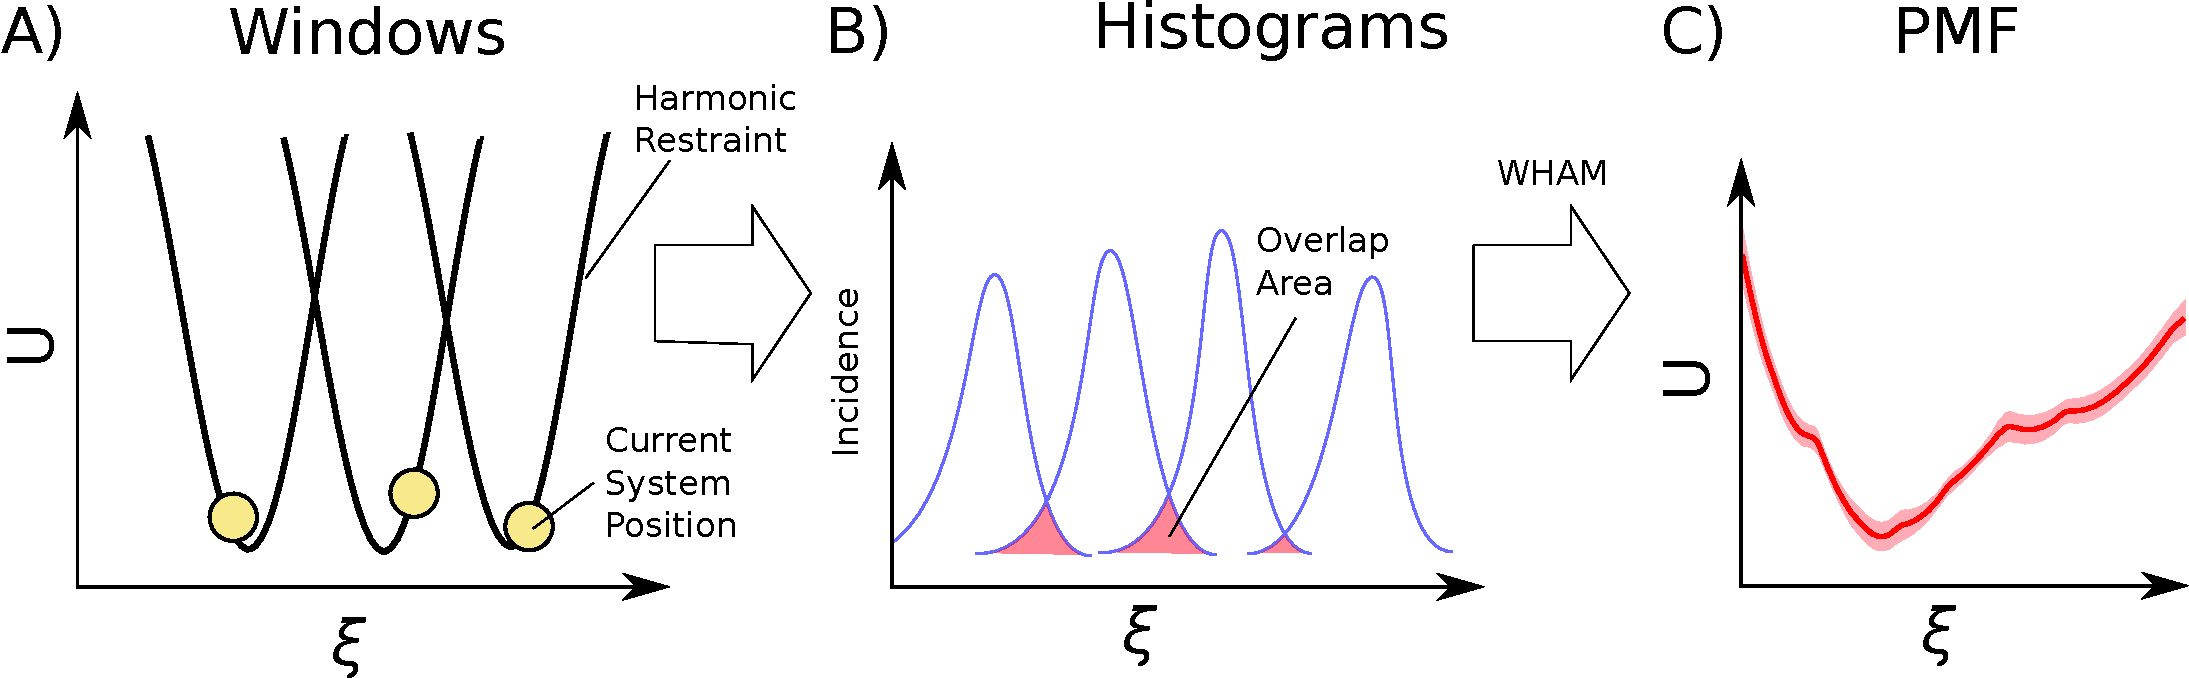
\includegraphics[width=\textwidth]{figures/umbrella_sampling.png.pdf}
	\end{center}
	\captionsetup{singlelinecheck = false, justification=raggedright}
	\caption[Illustration of Umbrella Sampling] {\textbf{Illustration of Umbrella Sampling}}{A) Several simulations are repeated with only one change. A bias  potential is added somewhere along the reaction coordinate $\xi$. B) The value of $\xi$ is recorded in each of the windows and then graphed as histograms. C) The Overlap in neighbouring histograms is integrated via the WHAM method to calculate the Potential of Mean Force. This gives us the energy landscape. Fluctuations in the overlap in the data can be used to estimate the error for the PMF. }
	\label{umbrella_sampling_illustration}
\end{figure}

This is 

\subsubsection{Weighted Histogram Average Method}

\subsection{Metadynamics}
